\section{Procedure di progetto}
\label{procedurediprogetto}

Quando non è specificato come modificare il valore di un parametro del ticket bisogna mantenere il valore già presente, o quello di default se il ticket è appena stato creato.

Il parametro ``Tag nel titolo'' corrisponde al testo racchiuso tra parentesi quadre che deve essere posto all'inizio del campo ``titolo'', in aggiunta al titolo esplicito.

\subsection{Creazione compito}

\begin{figure}[H]
    \centering
    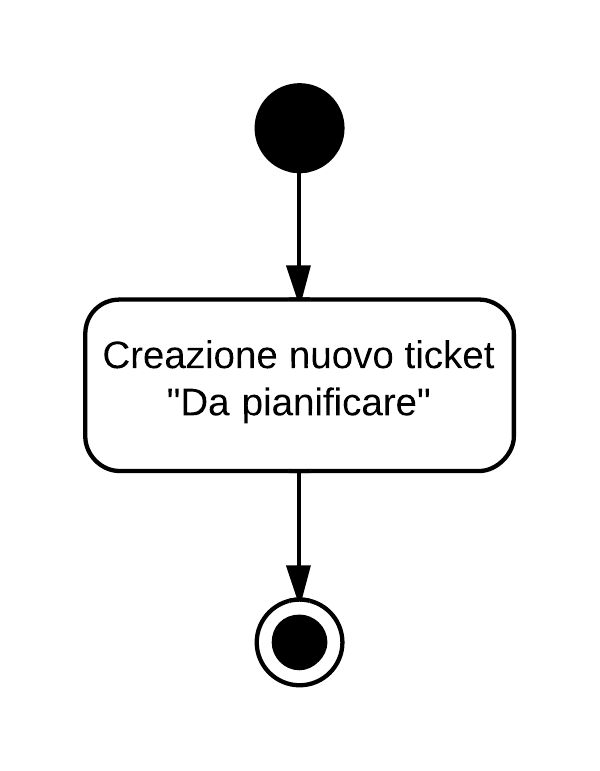
\includegraphics[width=7cm]{uml-processi/Creazione_compito.png}
    \caption{Creazione compito}
\end{figure}

Il Progettista, dopo aver completata la progettazione di dettaglio, deve creare i ticket di codifica con i seguenti parametri:
\begin{itemize}
 \item \textbf{Sezione}:''Da pianificare''
 \item \textbf{Milestone}: la revisione entro la quale il compito dovrà essere terminato.
 \item \textbf{Tag nel titolo}: nessuno.
 \item \textbf{Titolo}: breve descrizione del compito, con il riferimento all'unità di lavoro corrispondente.
 \item \textbf{Dipendenze}: le dipendenze decise nella progettazione.
 \item \textbf{Pianificazione}: nessuna.
 \item \textbf{Assegnato a}: il Responsabile.
\end{itemize}

\subsection{Pianificazione compito e verifica}
\label{pianificazione}

\begin{figure}[H]
    \centering
    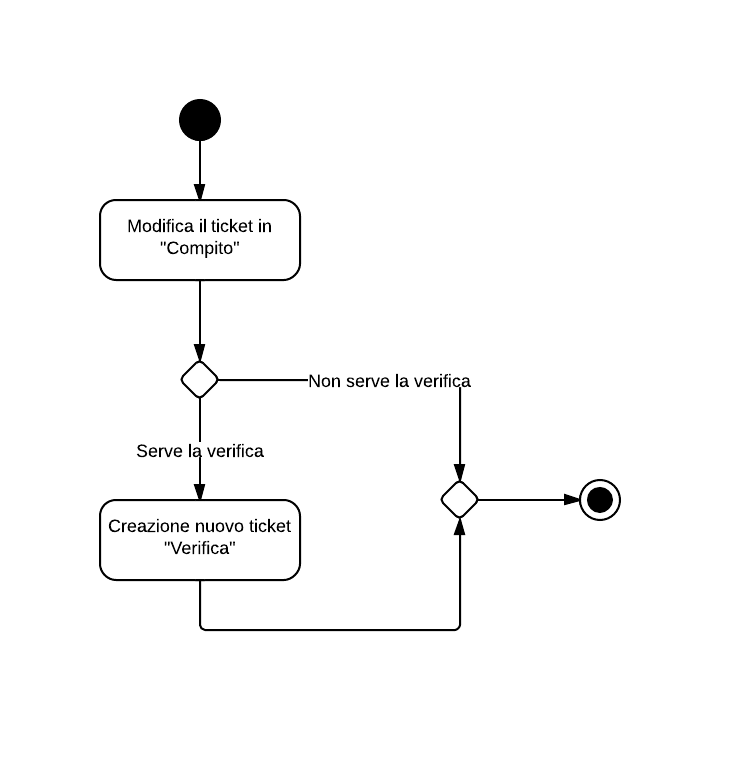
\includegraphics[width=11cm]{uml-processi/Pianificazione_compito_e_verifica.png}
    \caption{Pianificazione compito e verifica}
\end{figure}

Il Responsabile deve pianificare i ticket delle sezioni ``Da pianificare''. Deve inoltre creare e pianificare il corrispondente ticket di verifica se necessario. I ticket del compito e della modifica devono essere assegnati a persone diverse.

Modifica i parametri del compito:
\begin{itemize}
 \item \textbf{Sezione}: ``Compito''.
 \item \textbf{Pianificazione}: a scelta del Responsabile.
 \item \textbf{Assegnato a}: un programmatore, a scelta del Responsabile.
\end{itemize}

Parametri della verifica:
\begin{itemize}
 \item \textbf{Sezione}: ``Verifica''
 \item \textbf{Milestone}: la revisione entro la quale la verifica dovrà essere terminata.
 \item \textbf{Titolo}: breve descrizione della verifica, con un riferimento al compito da verificare.
 \item \textbf{Dipendenze}: il compito di cui bisogna fare la verifica.
 \item \textbf{Pianificazione}: a scelta del Responsabile.
 \item \textbf{Assegnato a}: un verificatore, a scelta del Responsabile.
\end{itemize}

\subsection{Esecuzione compito}

\begin{figure}[H]
    \centering
    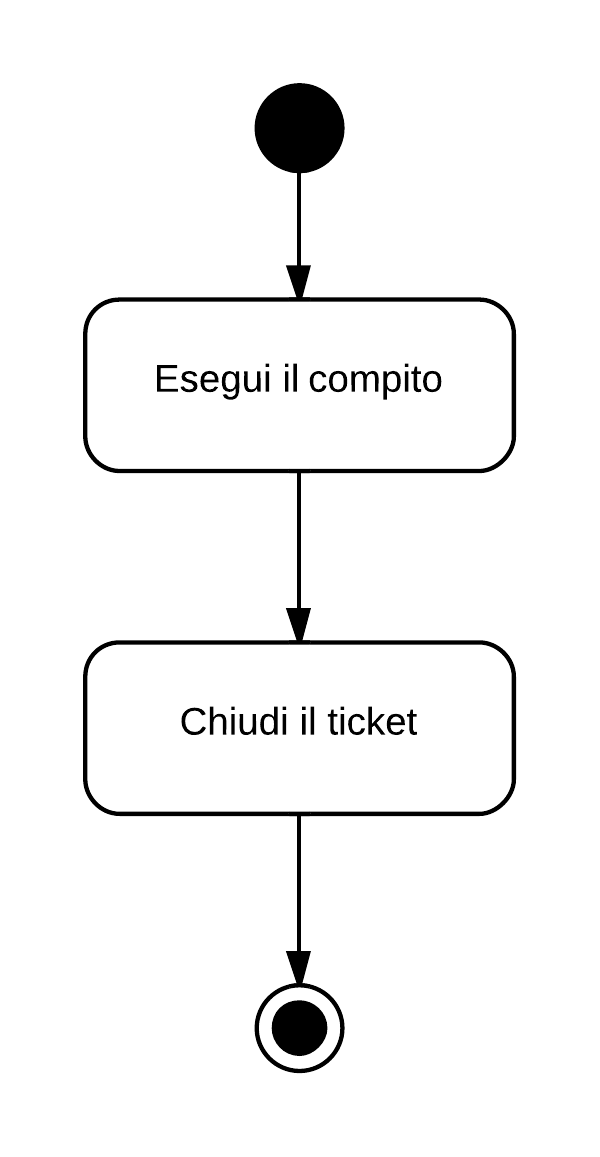
\includegraphics[width=7cm]{uml-processi/Esecuzione_compito.png}
    \caption{Esecuzione compito}
\end{figure}

Non appena il programmatore a cui è assegnato un ticket comincia a lavorare deve impostare una percentuale maggiore di $0\%$. Quando termina il compito deve chiudere il ticket:
\begin{itemize}
 \item \textbf{Stato}: ``Chiuso''.
\end{itemize}
 
\subsection{Esecuzione verifica}

\begin{figure}[H]
    \centering
    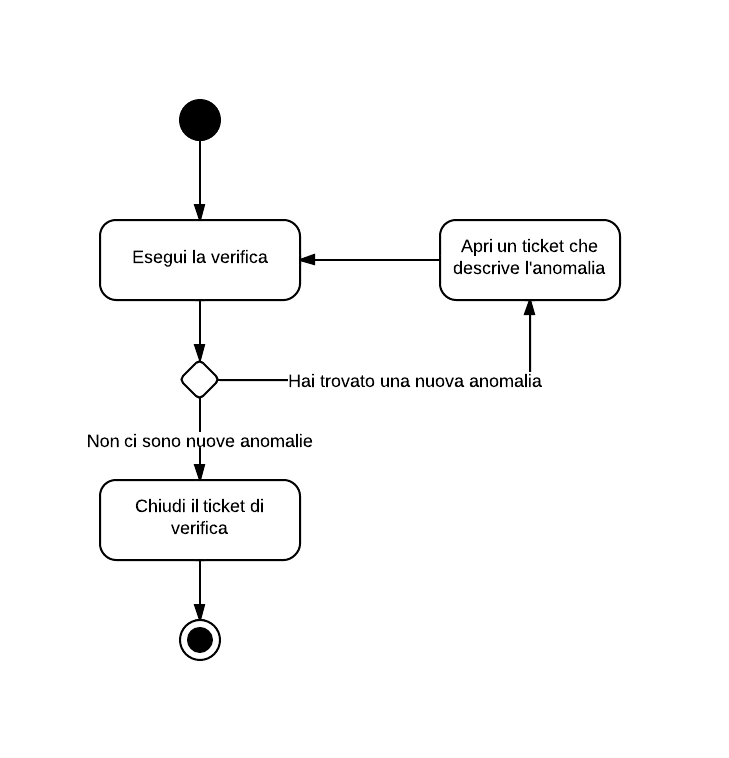
\includegraphics[width=11cm]{uml-processi/Esecuzione_verifica.png}
    \caption{Esecuzione verifica}
\end{figure}

Non appena il verificatore a cui è assegnato un ticket comincia a lavorare deve impostare una percentuale maggiore di $0\%$. Quando termina la verifica deve chiudere il ticket:
\begin{itemize}
 \item \textbf{Stato}: ``Chiuso''.
\end{itemize}

Nel caso in cui il verificatore trovi bug o non conformità significative deve creare un ticket di tipo ``Da valutare'':
\begin{itemize}
 \item \textbf{Sezione}: ``Da valutare''
 \item \textbf{Milestone}: la revisione entro la quale il bug dovrà essere corretto, è opzionale.
 \item \textbf{Tag nel titolo}: un aggettivo tra ``Error'', ``Fault'', ``Failure'', ``Mistake'', come descritto nel \PianoDiQualifica.
 \item \textbf{Titolo}: breve descrizione del bug, con un riferimento al compito nel quale lo si è trovato.
 \item \textbf{Dipendenze}: nessuna.
 \item \textbf{Pianificazione}: nessuna.
 \item \textbf{Assegnato a}: il Responsabile.
\end{itemize}

\subsection{Valutazione delle modifiche}

\begin{figure}[H]
    \centering
    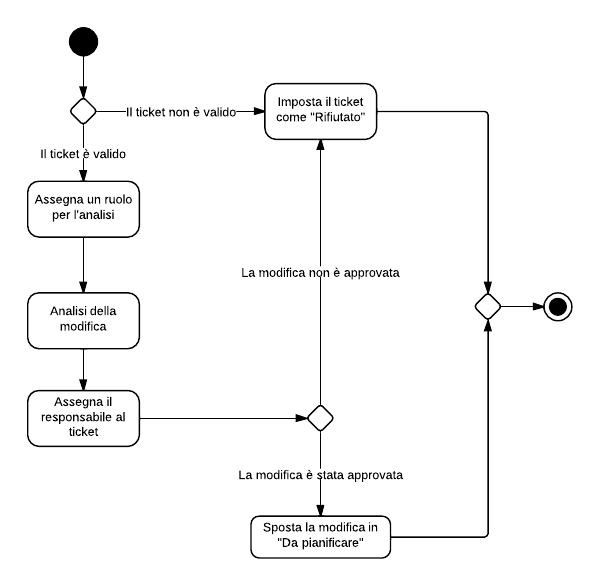
\includegraphics[width=1.2\textwidth]{uml-processi/Valutazione_delle_modifiche.png}
    \caption{Valutazione delle modifiche}
\end{figure}

Il Responsabile deve valutare ogni modifica del tipo ``Da valutare''. Se la formulazione della modifica è corretta allora la assegna ad un ruolo competente:
\begin{itemize}
 \item \textbf{Assegnato a}: un membro del gruppo a scelta del Responsabile
\end{itemize}

Tale ruolo, dopo averla analizzata, deve riassegnarla al Responsabile aggiungendo le informazione prodotte dall'analisi:
\begin{itemize}
 \item \textbf{Assegnato a}: il Responsabile
 \item \textbf{Descrizione}: la descrizione già presente con in aggiunta i risultati dell'analisi.
\end{itemize}

A questo punto, se il Responsabile ritiene che la modifica debba essere eseguita, imposta i seguenti parametri:
\begin{itemize}
 \item \textbf{Sezione}: ``Da pianificare''
 \item \textbf{Milestone}: la revisione entro la quale la modifica dovrà essere fatta.
\end{itemize}
e passa a pianificare il ticket, seguendo la procedura \ref{pianificazione}.

Se il Responsabile non approva o non è ritene valida la modifica deve impostare:
\begin{itemize}
 \item \textbf{Sezione}: ``Rifiutato''.
 \item \textbf{Assegnato a}: nessuno.
 \item \textbf{Stato}: ``Chiuso''.
\end{itemize}

\subsection{Richiesta di modifica e segnalazione bug}
\label{segnalazionebug}

\begin{figure}[H]
    \centering
    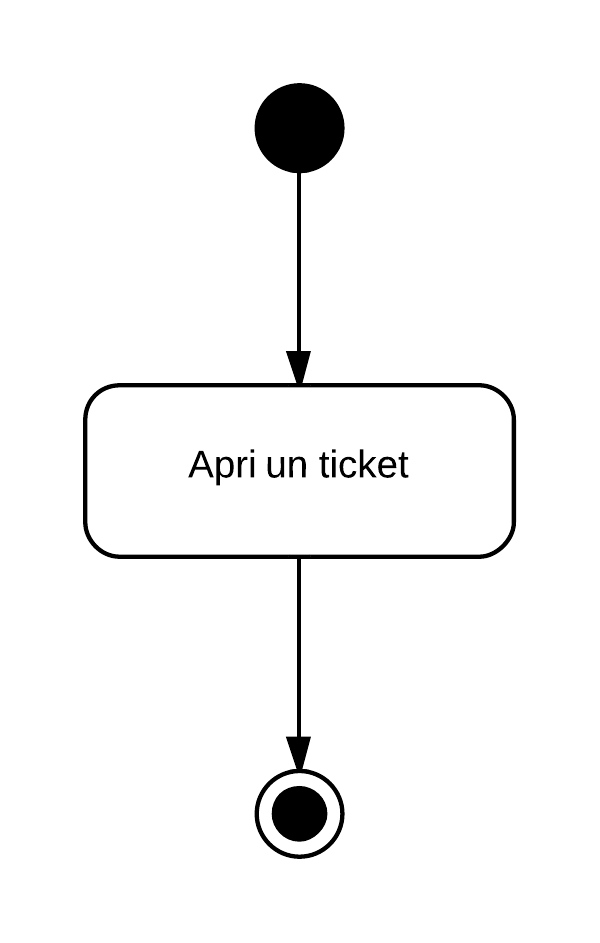
\includegraphics[width=7cm]{uml-processi/Richiesta_di_modifica_e_segnalazione_bug.png}
    \caption{Richiesta di modifica e segnalazione bug}
\end{figure}

Se un membro del gruppo volesse segnalare un bug o richiedere una modifica deve creare un ticket con i seguenti parametri:
\begin{itemize}
 \item \textbf{Sezione}: ``Da valutare''
 \item \textbf{Milestone}: la revisione entro la quale la modifica dovrà essere fatta, è opzionale.
 \item \textbf{Tag nel titolo}: un aggettivo tra ``Error'', ``Fault'', ``Failure'', ``Mistake'', come descritto nel \PianoDiQualifica, oppure ``Modifica'' se è una richiesta di modifica.
 \item \textbf{Titolo}: breve descrizione della modifica.
 \item \textbf{Descrizione}: descrizione completa e auto-sufficiente del bug o della modifica richiesta.
 \item \textbf{Dipendenze}: nessuna.
 \item \textbf{Pianificazione}: nessuna.
 \item \textbf{Assegnato a}: il Responsabile.
\end{itemize}
